\documentclass[titlepage]{article}
\usepackage{graphicx}



\author{ Dispoto, Brett\\
	\and
	Kamel, Adham\\
	\and
	Cai, Feiyu\\
}

\title{CS157A Project Proposal}

\begin{document}
	\maketitle
	
	\section{Project Overview}	
	%----------------------------------------Adham fill in here--------------------------
	%Provide descriptions of the three-tier Based Database Application your team will be developing. Who are stakeholders? Why is it important?   	
	



	\section{System Enviroment}
	
	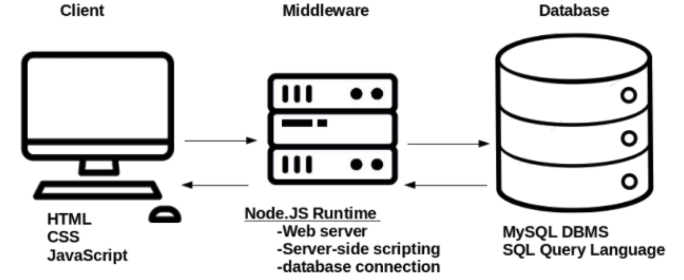
\includegraphics[scale=2.0]{3-tier.png}
	
	\subsection{Client}
		The presentation layer will be provided via the following languages/software:
	\begin{itemize}
		\item HTML
		\item CSS/Bootstrap
		\item JavaScript
		\item Web Browser 
	\end{itemize}
	\subsection{Middleware}
		All middleware will be provided via the Node.js Runtime Environment. This includes: 
	\begin{itemize}
		\item A server side scripting language (Node.js)
		\item Database connection via Node.js MySQL database driver	
		\item Node.js build-in web server (HTTP module)
	\end{itemize}
	
	\subsection{Relational Database}
		The relational database management system (RDBMS) in use will be MySQL, which will be queried via the Structured Query Language (SQL). The following data are examples of what will be stored:
	\begin{itemize}
		\item User information (name, DOB, username, password, site activity, favorites, etc)
		\item Book information (author, ISBN, publisher, date, reviews, etc)
	\end{itemize}

	\subsection{Hardware}
		Although this project will implement a three-tiered database application architecture, all three abstractions will be running on a single local host; this means that the architecture is only virtually three-tiered. 
	
	\section{Functional Requirements}
	The system will provide searching, sorting the shown book lists, reading books, reading reviews, and sharing via email functions from our free textbook database. 
	Anonymous visitors can use these functions without signing up for an account. However, signing up for an account with a valid email address will provide more functions. 
	A user can sign in his/her account with his/her email address and password. A sign in user will have additional functions such as writing reviews, setting favorite books and having access to their account details page. 
	

\textit{Supported features include:}
	\begin{itemize}
\item	\textbf{Reading:} reading the books itself or its reviews. Input: book information. Output: book content


\item	\textbf{Searching:} searching for book from the provided information. Input: title, author, year of publication, publisher, ISBN, genre, etc. Output: list of books fitting search query.
	
	
\item	\textbf{Sorting:} sort the way books are listed. Input: sorting rules such as reviews, alphabetical order, etc.
	
	
\item	\textbf{Review:} Give a review and write comments for a book. Input: review and comments. Output: Review and comments are posted on the database that everyone can see
	
	
\item	\textbf{Set favorites:} set a book as favorites, the user can see it in his/her profile. Input: “set favorites” button in book details. Output: books stores in the user’s profile.
	
	
\item	\textbf{Sharing via email:} sharing book details via email. Input: sharing button in book details. Output: generate share URL link that ready to send via email. 

	\end{itemize}



	\section{Non-functional Issues}
	\subsection{Graphical User Interface}
	The GUI of this project is focus on using mouse click and keyboard input to trigger the changes of content that will be displayed to user.
	\begin{itemize}
		\item Type of GUI: HTML/JavaScript based
		\item Software to build: Adobe XD
	\end{itemize}	
	\subsection{Access Control}
	There are two type of user with different access control:
	\begin{itemize}
		\item Admin: have control of all book contents, can edit, add, and delete books in additional to visitor users access.
		\item Visitor: Only have read access to website content and edit access to their own account. 
	\end{itemize}
	\subsection{Security}
	We planned to use SQL builed-in encryption method to encrypt user's information while storing into database. 




\end{document}
